\documentclass[12pt,a4paper]{article}
\usepackage[UTF8]{ctex}
\usepackage{graphicx}
\usepackage{geometry}
\usepackage{ulem}
\usepackage{enumitem}
\usepackage{titlesec}
\usepackage{multicol}
\usepackage[export]{adjustbox}
\usepackage{amsmath}  % 推荐用于更好的数学排版
\usepackage[utf8]{inputenc}
\usepackage{CJKutf8}
\usepackage{fancyhdr}
\usepackage{lastpage}
\usepackage{ulem}
\usepackage{tabularx}
\usepackage{float}
\usepackage{siunitx}
\usepackage{multirow} 

% 页眉页脚设置
\pagestyle{fancy}
\fancyhf{} % 清除所有页眉页脚
% 设置页眉内容
%-==========1. 填写从第二页开始 每页第一行的信息==========-
\fancyhead[C]{\small
    \makebox[4.5em][c]{实验名称：} \uline{\makebox[17em][c]{晶体管共射放大电路设计、仿真与测试}} 
    \makebox[2.5em][c]{姓名：} \uline{\makebox[4em][c]{}} 
    \makebox[2.5em][c]{学号：} \uline{\makebox[5em][c]{}}
}%--------------------------------------------------------
\fancyfoot[C]{\small 第 \thepage\ 页，共 \pageref{LastPage} 页}


% 取消页眉和页脚的下划线
\renewcommand{\headrulewidth}{0pt} % 页眉横线粗细设为0
\renewcommand{\footrulewidth}{0pt} % 页脚横线粗细设为0

% 调整页眉高度
\setlength{\headheight}{50pt}

% 设置plain样式（用于第一页）
\fancypagestyle{plain}{
    \fancyhf{} % 清除所有页眉页脚
    \renewcommand{\headrulewidth}{0pt} % 隐藏页眉横线
    \fancyfoot[C]{第 \thepage\ 页，共 \pageref{LastPage} 页} % 保留页脚
}
% 设置页面边距
\geometry{left=2.54cm,right=1.5cm,top=2.54cm,bottom=2.54cm}

% 设置正文字体大小为小四
\renewcommand{\normalsize}{\fontsize{12pt}{16pt}\selectfont}
% 设置章节格式
\titleformat{\section}{\fontsize{16pt}{22pt}\selectfont\bfseries}{\thesection}{1em}{} % 一级标题：三号
\titleformat{\subsection}{\fontsize{15pt}{20pt}\selectfont\bfseries}{\thesubsection}{1em}{} % 二级标题：小三

\begin{document}
\thispagestyle{plain}%第一页使用 plain 样式，而不是默认的 fancy 样式，第一页不再显示页眉
% 标题部分 - 两栏布局
\begin{multicols}{2}
    % 左栏：图片和实验报告标题
    % 左栏：使用空行创建前三行
    \noindent
    ~\\ % 第一行
    ~\\ % 第二行
    ~\\ % 第三行
    \hphantom{占位}% 使用空占位符
    \raisebox{-0.5\baselineskip}% 图片向下移动半行
    {
\includegraphics[width=1.85in,height=0.58in]{ZJU.jpg}}
    \hspace{.5em}% 图片和标题之间的间距
    \raisebox{0pt}[\height][0pt]% 标题底部对齐
    {\textbf{\fontsize{26pt}{30pt}\selectfont 实验报告}}
    
    \columnbreak % 换到右栏
    
    % 右栏：个人信息
    % 右栏：个人信息 - 靠右对齐 
%-==========2. 填写个人信息==========-
    \begin{flushright}
        \small
        \makebox[3em][l]{专业：} \uline{\makebox[9em][c]{法语-电子科学与技术}} \\
        \makebox[3em][l]{姓名：} \uline{\makebox[9em][c]{}} \\
        \makebox[3em][l]{学号：} \uline{\makebox[9em][c]{}} \\
        \makebox[3em][l]{日期：} \uline{\makebox[9em][c]{2025年12月2/9日}} \\
        \makebox[3em][l]{地点：} \uline{\makebox[9em][c]{紫金港东四216}} \\
    \end{flushright}   
\end{multicols}
% 课程名称等信息（单栏）
%-==========3. 填写课程信息==========-

{\small
\noindent
课程名称： \uline{电子电路设计实验I} \hfill 指导老师： \uline{施红军、叶险峰、邓靖靖} \hfill 成绩： \uline{\hspace{3cm}} \\
实验名称：\uline{晶体管共射放大电路设计、仿真与测试}\hfill 实验类型：\uline{设计实验}\hfill 同组学生姓名：\uline{}
}
%-==========4. 正文开始==========-
\section*{一、实验目的}

学习晶体管放大电路的设计方法，掌握晶体管放大电路静态工作点的设置、测量与调整方法，了解放大器的非线性失真，掌握放大器电压增益、输入电阻、输出电阻、幅频响应等基本性能指标的测量方法，理解负反馈对放大电路性能的影响。


\section*{二、实验任务与要求}

1、设计一阻容耦合单级放大电路

已知条件：$V_{CC} = +\SI{+10}{\volt}$，$R_L = \SI{5.1}{\kilo\ohm}$，$V_i = \SI{10}{\milli\volt}$，$R_s = \SI{600}{\ohm}$

性能指标要求：$f_L < \SI{30}{\hertz}$，对频率为 $\SI{1}{\kilo\hertz}$ 的正弦信号 $|A_v| > 15$，$R_i > \SI{7.5}{\kilo\ohm}$

2、设计要求

（1）写出详细设计过程并进行验算

（2）用软件进行仿真

3、电路安装、调整与测量

编写调试步骤,设计数据记录表格，对放大电路特性进行测试：

（1）静态工作点的调整和测量

（2）电压增益的测量

（3）输入电阻、输出电阻的测量

（4）上限截止频率\( f_H \)、下限截止频率\( f_L \)的测量



4、写出设计性实验报告


\section*{三、实验原理}

\subsection*{1、晶体管共射放大电路分析计算}

\begin{figure}[H]
    \centering
    
\includegraphics[width=0.5\textwidth, height=0.2\textheight]{1.png}
    \caption{带射极负反馈的共射放大电路}
    \label{fig1}
\end{figure}


图\ref{fig1}是一个带射极负反馈的共射放大电路。其中 \( R_{1} \)、\( R_{2} \) 提供静态工作点所需基极电压；\( R_{P} \) 进行静态工作点的调节；\( R_{A} \) 保护电路，避免 \( R_P\) 调至0时基极电流过大，损坏晶体管；\( R_C \) 为直流负载电阻，\( R_L \) 为交流负载电阻，\( C_1 \)、\( C_2 \) 为耦合电容。其中 \( R_{E1} \)、\( R_{E2} \) 都参与直流电流负反馈，但只有 \( R_{E1} \) 参与交流电流负反馈（旁路电容 \( C_E \) 交流短路）。

\begin{figure}[H]
    \centering
    
\includegraphics[width=0.35\textwidth, height=0.2\textheight]{2.png}
    \caption{直流通路及其戴维南等效电路}
    \label{fig2}
\end{figure}

在如图\ref{fig2}所示的戴维南等效电路中，有
\[  
\begin{cases}
V_{BB} = V_{CC} \dfrac{R_{2}}{R_{1} + R_{2}}, \\
R_{BB} = R_{1} \parallel R_{2}, 
\end{cases}
\]

对电路进行直流分析，有
\[
\begin{cases}
I_C = \dfrac{\beta}{1+\beta} I_B \approx I_E, \\
V_{CE} \approx V_{CC} - (R_C + r_{be}) I_C, \\
I_E = \dfrac{V_{BB} - V_{BE}}{r_{be} + \dfrac{R_{BB}}{1-\beta}}
\end{cases}
\]

交流小信号参数
\[
\begin{cases}
g_m = \dfrac{I_C}{V_T} \\
r_{\pi} = \dfrac{\beta}{g_m} \\
r_{be} \approx \dfrac{1}{g_m}
\end{cases}
\]

对电路进行交流分析，等效电路图如下：



\begin{figure}[H]
    \centering
    
\includegraphics[width=0.4\textwidth, height=0.14\textheight]{3.png}
    \caption{交流通路}
    \label{fig3}
\end{figure}

电压增益 \( A_v \)
\[
A_v = -\frac{v_o}{v_i} \approx -\frac{R'_C}{R_E} = -\frac{R_C \parallel R_L}{r_e + R_{E1}}\]

输入电阻 \( R_i \) 
\[
R_i = R_1 \parallel R_2 \parallel \left[ (1 + \beta) \left( r_e + R_{E1} \right) \right]\]

输出电阻 \( R_o \)
\[
R_o \approx R_C\]

下限截止频率\( f_L \) 
\[
f_L \approx \frac{1}{2\pi} \sqrt{\omega_{C1}^2 + \omega_{C2}^2 + \omega_{CE}^2}\]

其中
\[
\omega_{C1} = \frac{1}{(R_S + R_i)C_1}\]
\[
\omega_{C2} = \frac{1}{(R_C + R_L)C_2}\]
\[
\omega_{CE} = \frac{1}{\left[ R_{E2} \parallel \left( R_{E1} + r_e + \frac{R_s \parallel R_1 \parallel R_2}{1 + \beta} \right) \right] C_E}\]

且当这三个电容值相当时，\( f_L \) 主要由旁路电容 \( C_E \) 引入的转折频率决定。

\subsection*{2、静态工作点与失真}
\begin{figure}[H]
    \centering
    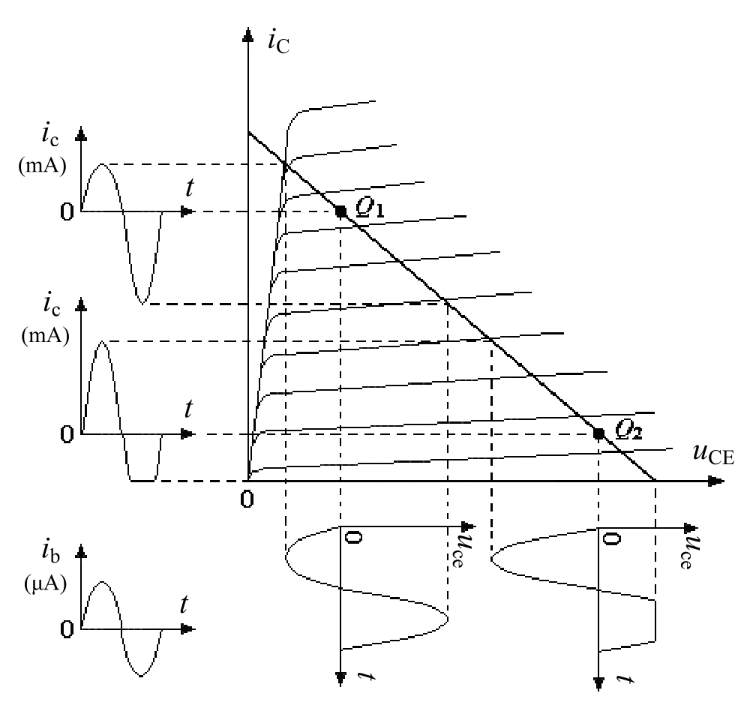
\includegraphics[width=0.5\textwidth, height=0.3\textheight]{99.png}
    \caption{静态工作点选择不当产生的非线性失真}
    \label{fig99}
\end{figure}

静态工作点选得过高或过低都易产生非线性失真。

若工作点过高（如 \( Q_1 \)），稍大的输入信号正半周将使晶体管进入饱和区，因而 \( i_c \) 波形将出现顶部压缩，输出电压 \( v_{CE} \) 波形将在底部压缩，出现\textbf{饱和失真}。

若工作点过低（如 \( Q_2 \)），稍大的输入信号负半周将使晶体管进入截止区，因而 \( i_c \) 波形将出现底部削平，输出电压 \( v_{CE} \) 波形将在顶部削平，出现\textbf{截止失真}。

因此，要使放大器不失真地放大，工作点必须选择合适。初选静态工作点时，可以选取直流负载线的中点，即 
\[
V_{CE} = 0.5V_{CC} \quad \text{或} \quad I_C = 0.5I_{CS},
\] 
这样便可获得较大输出动态范围。当放大器输出端接有负载 \( R_L \) 时，因交流负载线比直流负载线要陡，所以放大器动态范围要变小。当发射极接有电阻时，也会使信号动态范围变小。

\section*{四、实验方案设计与参数计算}

\subsection*{4.1 实验电路}

实验电路如图\ref{fig4}所示。晶体管选用2N2222，\(\beta=120\)。

\begin{figure}[H]
    \centering
    
\includegraphics[width=0.5\textwidth, height=0.2\textheight]{1.png}
    \caption{实验电路}
    \label{fig4}
\end{figure}

且已知$V_{CC} = +\SI{+10}{\volt}$，$R_L = \SI{5.1}{\kilo\ohm}$，$V_i = \SI{10}{\milli\volt}$，$R_s = \SI{600}{\ohm}$

性能指标要求：$f_L < \SI{30}{\hertz}$，对频率为 $\SI{1}{\kilo\hertz}$ 的正弦信号 $|A_v| > 15$，$R_i > \SI{7.5}{\kilo\ohm}$

\subsection*{4.2 参数计算}



\subsubsection*{(1) 静态工作点}
由于被测信号幅度较小，考虑噪声因素，取晶体管静态电流为
\[
I_C = 1 \,\text{mA}
\]
取
\[
V_B = \frac{1}{4} V_{CC} = 2.5 \,\text{V}
\]
则
\[
R_E \approx \frac{V_B - V_{BE}}{I_C} = 1.8 \,\text{k}\Omega
\]
当 \( I_R \gg I_B \) 时，\( V_{BB} \approx V_B = 2.5 \,\text{V} \)，由 \( V_{BB} \) 表达式可得：
\[
10 \times \frac{R_2}{R_1 + R_2} = 2.5 \quad \Rightarrow \quad R_1 : R_2 = 3 : 1
\]


    从输入电阻要求来看，一般\(R_2\)取三倍\(R_i\)下界，取 \[ R_2 = 22.5 \,\text{k}\Omega , R_1 = 67.5 \,\text{k}\Omega \]


对应标称值 \[ R_2 = 22 \,\text{k}\Omega , R_1 = 68 \,\text{k}\Omega \]

为使静态工作点易调，\( R_1 \) 可由 43 kΩ 固定电阻与 50 kΩ 电位器串联构成。

\subsubsection*{(2) 动态参数}
由 \( I_C = 1 \,\text{mA} \) 得
\[
r_e \approx 26 \,\Omega
\]
取 \( |A_V| = 20 \,\text{V/V} \)，由增益表达式得：
\[
\frac{R_C \parallel 5.1 \,\text{k}\Omega}{26 + R_{E1}} = 20
\]

从输入电阻出发，取 \( R_i = 8 \,\text{k}\Omega \)，可得
    \[
    R_{E1} = 101.44 \,\Omega, \quad R_C = 5.095 \,\text{k}\Omega, \quad R_{E2} = 1698.56 \,\Omega
    \]
    
对应标称值 \[ R_C = 5.1 \,\text{k}\Omega , R_{E1} = 100 \,\Omega,R_{E2} = 1.6 \,\text{k}\Omega \]

\subsubsection*{(3) 电容}
取 \( f_L = 30 \,\text{Hz} \)，则
\[
C_E = \frac{1}{2\pi f_L \left[ R_{E2} \parallel \left( R_{E1} + r_e+\frac{R_s\parallel R_1\parallel R_2}{1+\beta} \right) \right]} \approx 43.9 \,\mu\text{F} \quad \text{（取 } 47 \,\mu\text{F} \text{）}
\]
\( C_1, C_2 \) 取标称值 \( 10 \,\mu\text{F} \)。

\subsubsection*{(4) 验算}
由\(
R_1 = 68 \,\text{k}\Omega, R_2 = 22 \,\text{k}\Omega, R_C = 5.1 \,\text{k}\Omega,  R_{E1} = 100 \,\Omega,  R_{E2} = 1.6 \,\text{k}\Omega
,
C_1 = C_2 = 10 \,\mu\text{F}, C_E = 47 \,\mu\text{F}, V_{CC} = 10 \,\text{V}
\),计算得到
\[
I_C = 1.026 \,\text{mA},  \quad |A_V| = 20.35 \,\text{V/V}, \quad R_i = 7.90 \,\text{k}\Omega, \quad R_o = 5.1 \,\text{k}\Omega,\quad f_L = 28.17 \,\text{Hz}
\]

\section*{五、实验仪器设备}

直流稳压电源、信号源、示波器。

\section*{六、实验步骤、调试过程、实验数据记录}

\subsection*{6.1 电路仿真}

在OrCAD中，绘制如图所示电路图。

\begin{figure}[H]
    \centering
    
\includegraphics[width=0.5\textwidth, height=0.22\textheight]{6.png}
    \caption{OrCAD仿真电路}
    \label{fig6}
\end{figure}

\subsubsection*{6.1.1 静态工作点}

在仿真设置中，选择时域分析，并进行参数设置。运行仿真，可得静态工作点参数
\[I_c=\frac{10-4.958}{5.1\text{k}}=0.989\text{mA},\quad V_{CE}=3.266\text{V}, \quad V_{BE}=0.645\text{V}\]


在仿真波形窗口中新增坐标（\(V_o\)和\(V_i\)），得到如下波形。可得出放大倍数\(A_v\)接近20。


\begin{figure}[H]
    \centering
    
\includegraphics[width=0.7\textwidth, height=0.3\textheight]{8.png}
    \caption{输入和输出电压仿真波形}
    \label{fig8}
\end{figure}

\subsubsection*{6.1.2 放大倍数}

在仿真设置中，选择交流分析，并进行参数设置。运行仿真，在仿真波形窗口中新增坐标（\(V_o/V_i\)）得到电压增益频率响应曲线。

\begin{figure}[H]
    \centering
    
\includegraphics[width=0.7\textwidth, height=0.3\textheight]{10.png}
    \caption{电压增益频率响应仿真波形}
    \label{fig10}
\end{figure}

启用光标，并将光标移至1kHz，读出\(A_v=19.940\text{V/V}\)。

\begin{figure}[H]
    \centering
    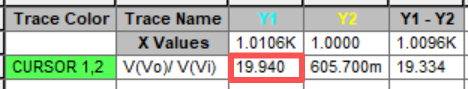
\includegraphics[width=0.45\textwidth, height=0.06\textheight]{81.png}
    \caption{光标读出放大倍数\(f_L\)}
    \label{fig81}
\end{figure}

\subsubsection*{(3)上限频率和下限频率}

为了得出上限频率\(f_H\)和下限频率\(f_L\)，将坐标改为DB\((V_o/V_i\))。

\begin{figure}[H]
    \centering
    
\includegraphics[width=0.7\textwidth, height=0.3\textheight]{11.png}
    \caption{电压增益频率响应仿真波形（DB）}
    \label{fig11}
\end{figure}


从峰值向下读3dB，得出上限频率\(f_H = 13.103 \,\text{MHz}\),下限频率\(f_L = 29.634 \,\text{Hz}\)。
\begin{figure}[H]
    \centering
    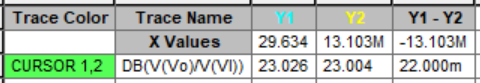
\includegraphics[width=0.45\textwidth, height=0.06\textheight]{12.png}
    \caption{光标读出上限频率\(f_H\)和下限频率\(f_L\)}
    \label{fig12}
\end{figure}

基极-集电极电容\(C_u\)会通过\textbf{密勒效应}在输入端产生一个等效电容 
\[
C_M = C_u (1 + |A_v|)
\] 
这会大幅降低高频截止频率 \( f_H \)。

改变 \( C_u \) 的值，可以直接观察到 \( f_H \) 的变化。
\begin{table}[H]
\centering
\caption{不同\(C_u\)值对应的\(f_H\)值} 
\renewcommand{\arraystretch}{1.2}
\small
\begin{tabular}{|p{1.6cm}|p{1.4cm}|p{1.4cm}|p{1.4cm}|p{1.4cm}|}
\hline

\(C_u\)/pF &不加 &0.01 &104 &134   \\
\hline
\(f_H\)/Hz &13.14M &13.11M &578.57k &453.46k   \\
\hline

\end{tabular}

\end{table}

\subsubsection*{6.1.3 输入电阻}

将\(R_L\)开路，运行仿真。在仿真波形窗口中新增坐标（\(V_i/I_{V1}\)），得到如下波形。

\begin{figure}[H]
    \centering
    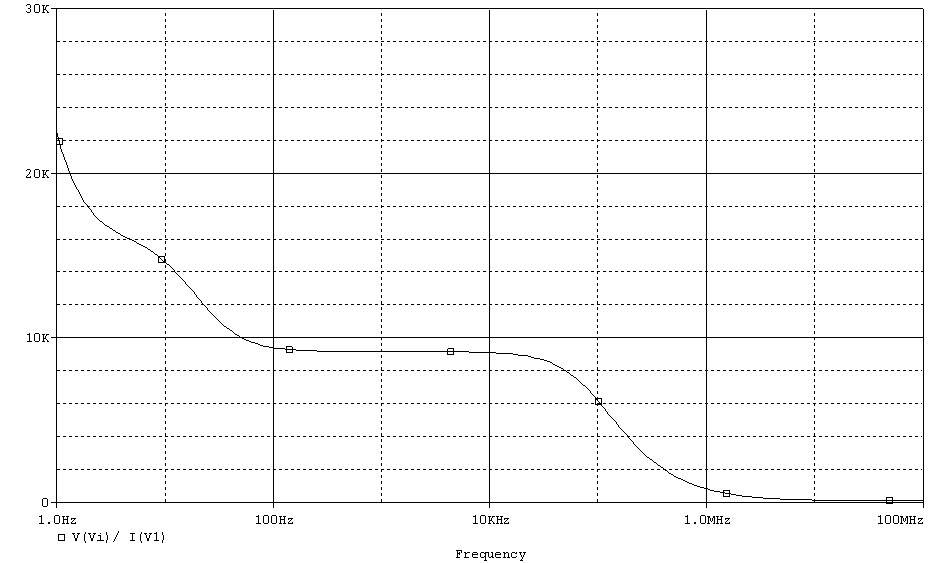
\includegraphics[width=0.7\textwidth, height=0.3\textheight]{21.png}
    \caption{输入电阻频率响应仿真波形}
    \label{fig21}
\end{figure}

启用光标，并将光标移至1kHz，读出输入电阻\(R_i=9.1462 \,\text{k}\Omega\)。

\begin{figure}[H]
    \centering
    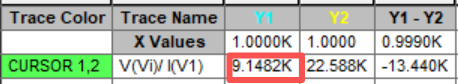
\includegraphics[width=0.45\textwidth, height=0.06\textheight]{22.png}
    \caption{光标读出输入电阻\(R_i\)}
    \label{fig22}
\end{figure}



\subsubsection*{6.1.4 输出电阻}

将输入电压源Turn off，并将\(R_L\)替换成电压源，运行仿真。在仿真波形窗口中新增坐标（\(V_o/I_{V1}\)），得到如下波形。

\begin{figure}[H]
    \centering
    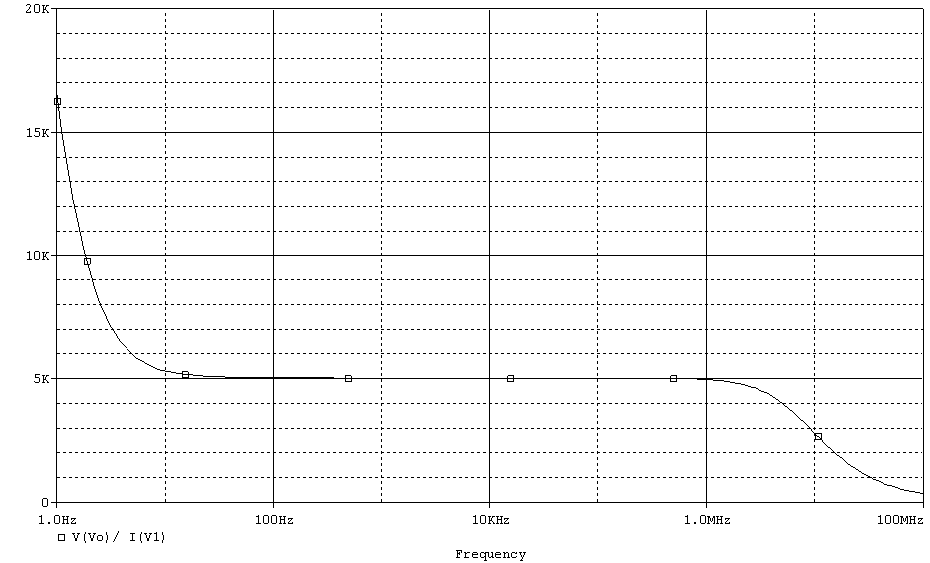
\includegraphics[width=0.7\textwidth, height=0.3\textheight]{23.png}
    \caption{输出电阻频率响应仿真波形}
    \label{fig23}
\end{figure}

启用光标，并将光标移至1kHz，读出输出电阻\(R_o=5.0299 \,\text{k}\Omega\)。
\begin{figure}[H]
    \centering
    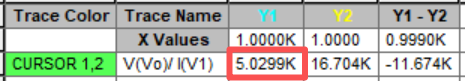
\includegraphics[width=0.45\textwidth, height=0.06\textheight]{24.png}
    \caption{光标读出输出电阻\(R_o\)}
    \label{fig24}
\end{figure}




\subsection*{6.2 电路测试}

\subsubsection*{6.2.1 静态工作点的调整和测量}



（1）按电路图安装元件，$C_u$暂不插入；

（2）连接直流电源，调整$V_{CC}$至预设值；

（3）开关切至ON，观察各极电压；

（4）调节$R_W$使$I_C$达到设计值；

\begin{figure}[H]
    \centering
    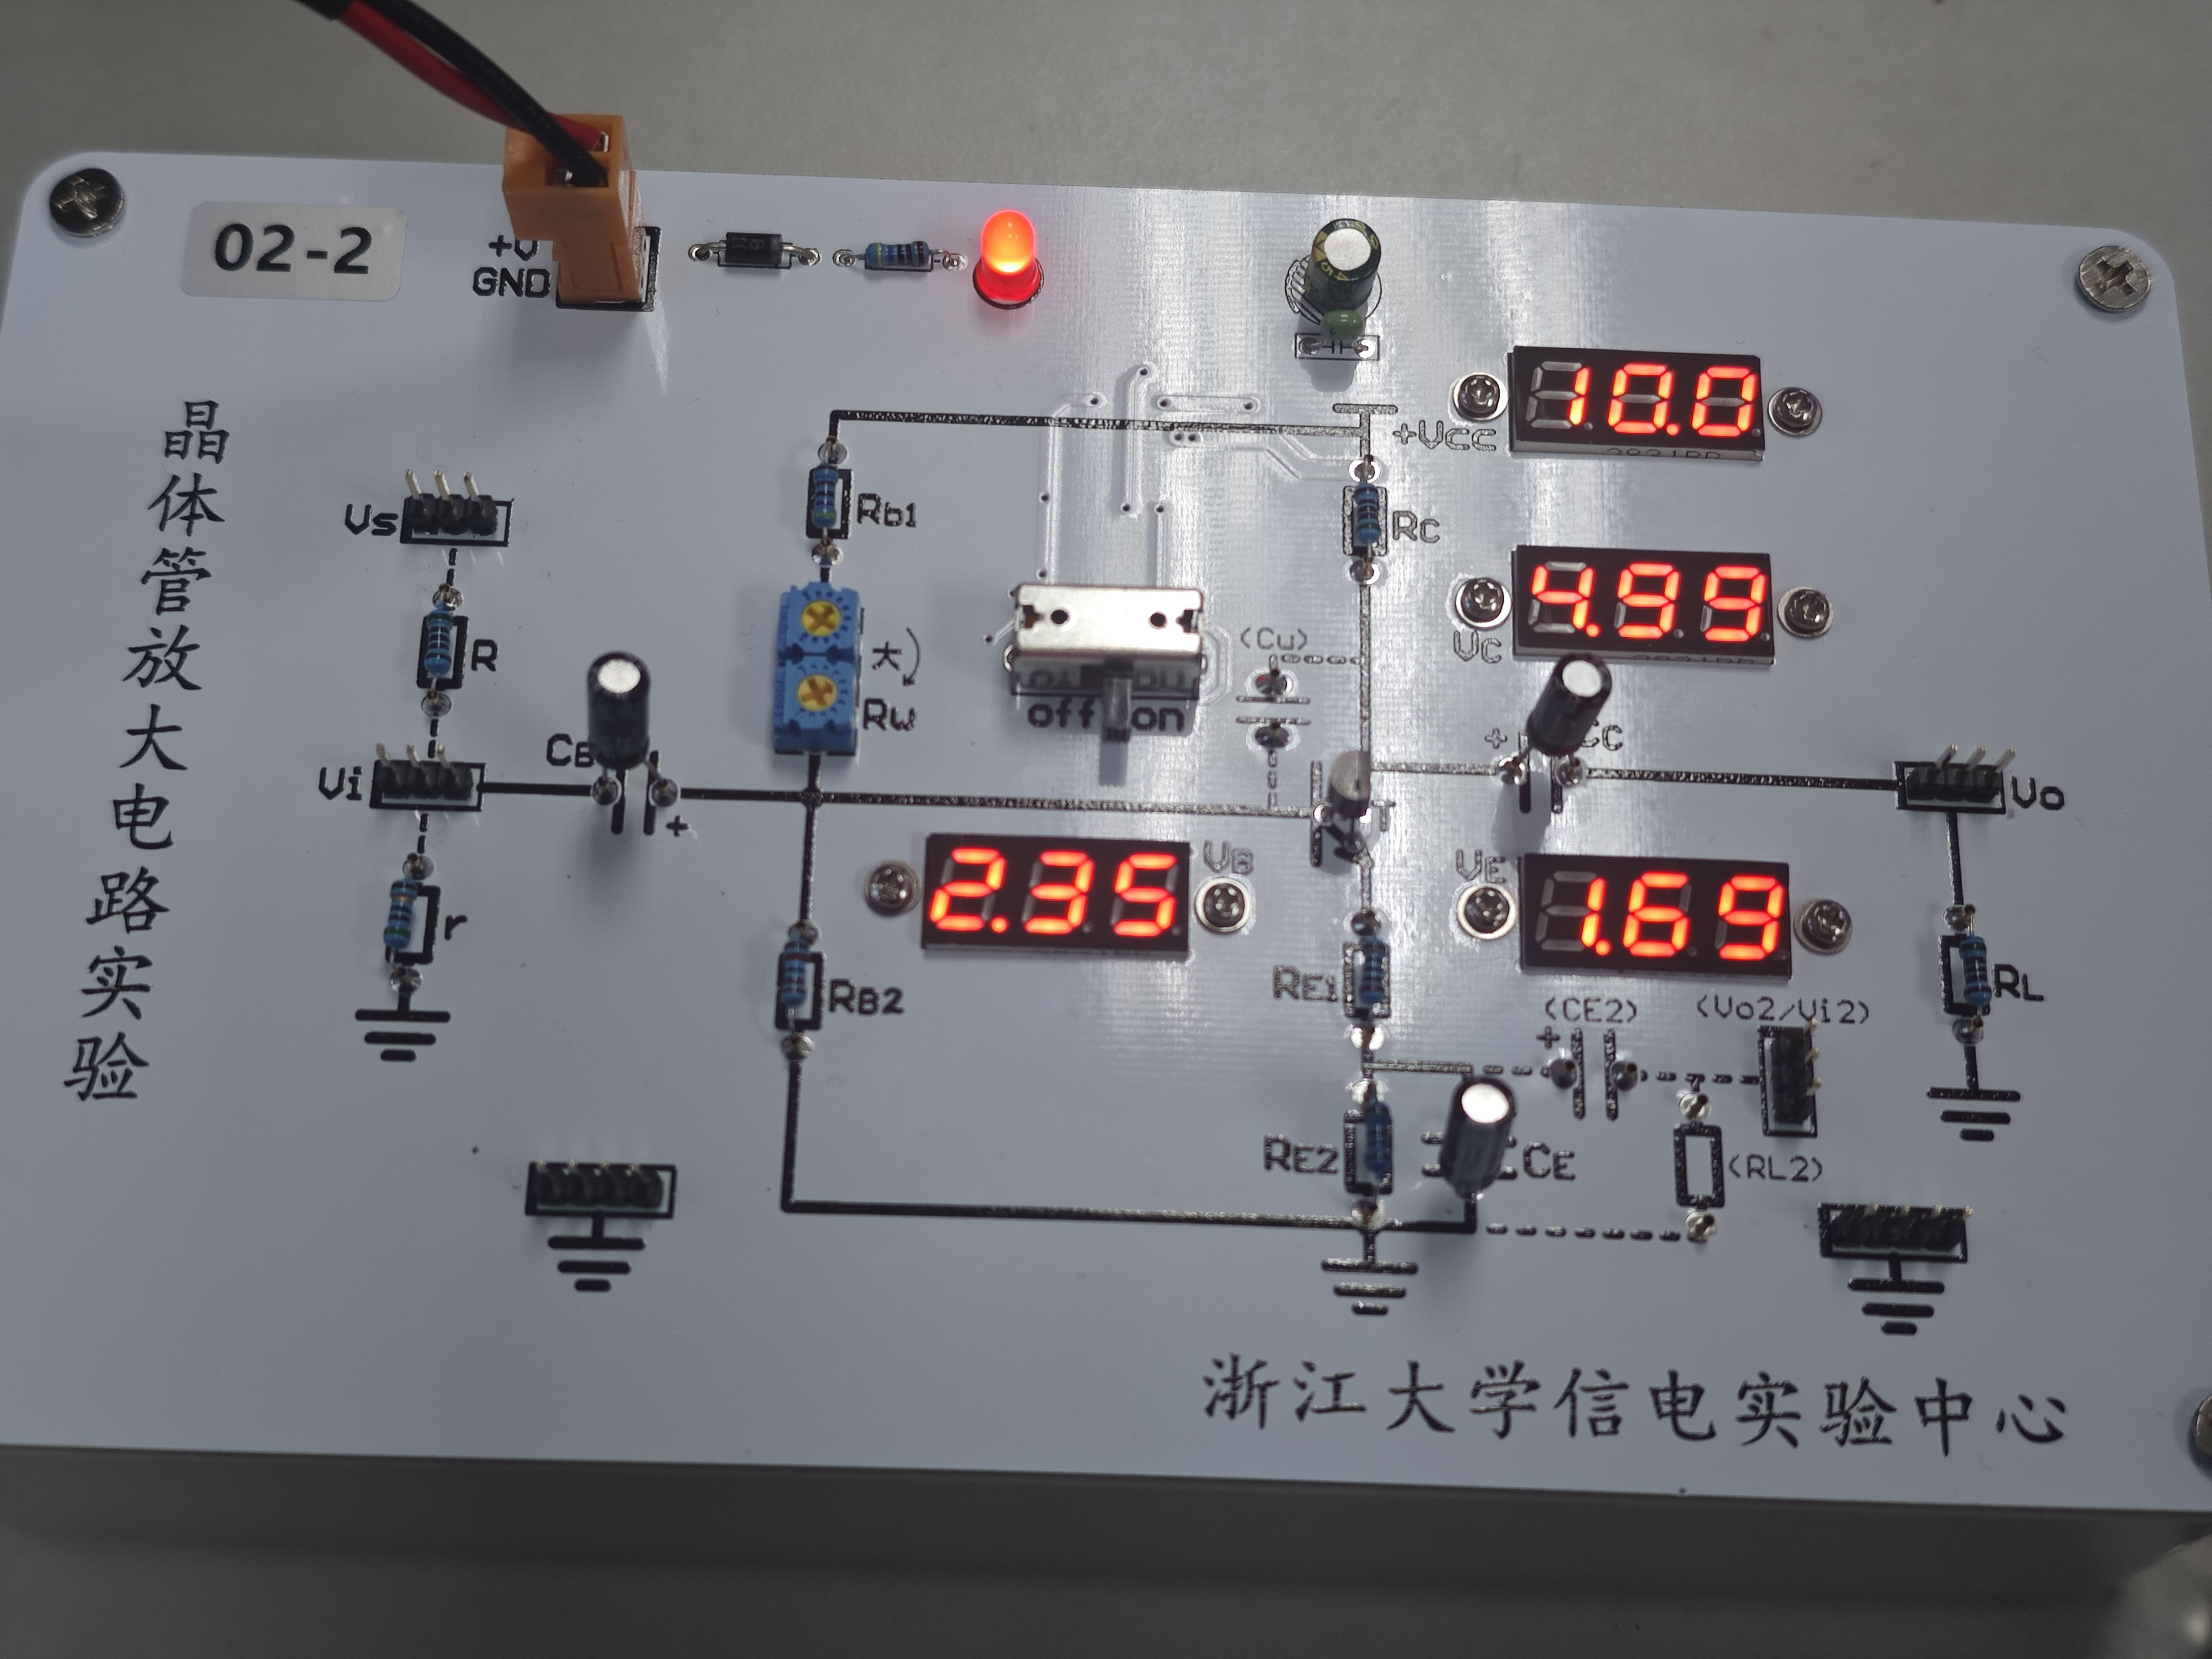
\includegraphics[width=0.45\textwidth, height=0.2\textheight]{40.jpg}
    \caption{静态工作点调整完毕}
    \label{fig40}
\end{figure}

（5）测量并记录静态工作点数据。

\begin{table}[H]
\centering
\caption{静态工作点数据记录}
\begin{tabular}{|c|c|c|c|c|c|}
\hline
 & $I_C$ (mA) & $V_{CE}$ (V) & $V_{BE}$ (V) & $V_B$ (V) & 工作状态判断 \\
\hline
理论估算值 &0.988 & 3.266&0.645 & 2.337& \multirow{2}{*}{放大} \\
\cline{1-5}
测量值 &0.982 & 3.30& 0.66& 2.35& \\
\hline
\end{tabular}
\end{table}

（6）测量完成后，开关切至OFF，断开显示电路。

\subsubsection*{6.2.2 电压增益测量}

（1）输入2kHz、10mV正弦信号，示波器观察波形相位；

（2）不接入输出电阻，即$R_L = \infty$，测量$v_i$、$v_o$（有$C_E$）；

（3）拔出$C_E$，再次测量$v_o$；

（4）增大输入信号至输出失真，记录失真类型及最大不失真输出电压；失真为\textbf{顶部失真（截止失真）}，此时输出的最大
值和最小值的绝对值之差超过了0.3V。同时可以观察到输出和输入呈\textbf{反相关系}。

\begin{figure}[H]
    \centering
    
\includegraphics[width=0.7\textwidth, height=0.3\textheight]{41.png}
    \caption{出现失真}
    \label{fig41}
\end{figure}

（5）接入$R_L = 5.1k\Omega$，测量$v_o$。


\begin{table}[H]
\centering
\caption{电压增益测量数据}
\begin{tabular}{|c|c|c|c|c|c|}
\hline
\textbf{测试条件} & $V_{iP-P}$ (mV) & $V_{oP-P}$ (V) & $V_{oP-Pmax}$ (V) & $|A_v|$ (实测) & $|A_v|$ (理论) \\
\hline
$R_L = \infty$，有$C_E$ & 20 & 764.56&5.9 &38.228 & 39.583\\
\hline
$R_L = \infty$，无$C_E$ & 20 & 58.786& -- &2.939 & 2.931\\
\hline
$R_L = 5.1k\Omega$，有$C_E$ & 20 & 387.16& -- &19.358 & 19.940\\
\hline
\end{tabular}
\end{table}


\subsubsection*{6.2.3 输入电阻测量}

在输出波形不失真的情况下，串联已知电阻$R$（与$R_i$同数量级）于信号源与放大器之间，测量$v_s$和$v_i$，计算

\[R_i = \dfrac{v_i}{v_s - v_i} \times R\]

\begin{figure}[H]
    \centering
    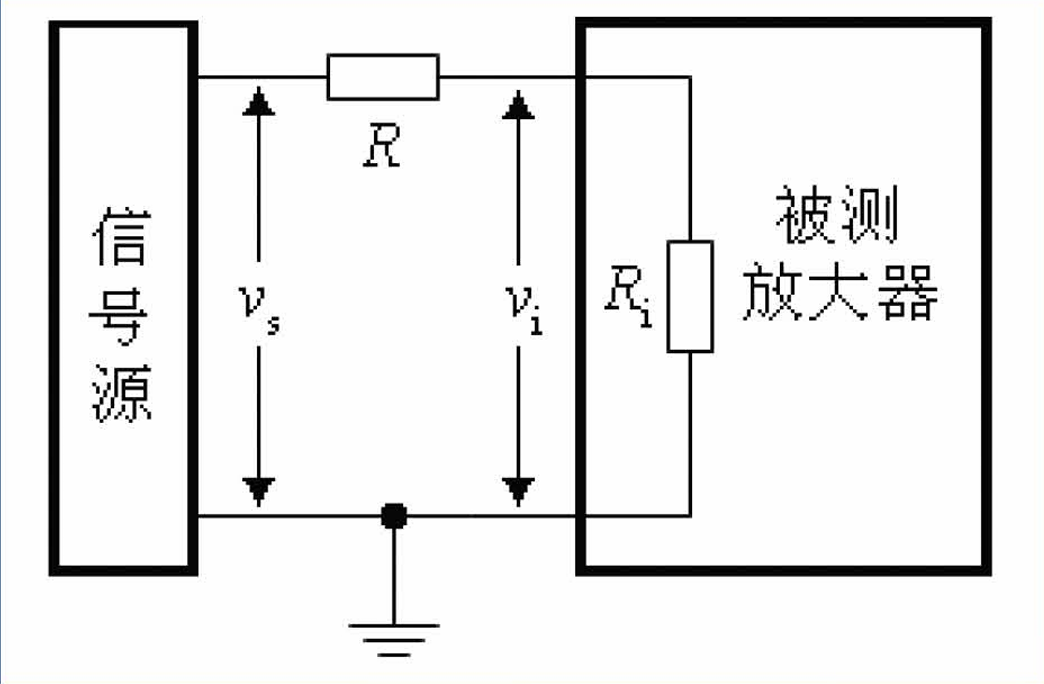
\includegraphics[width=0.4\textwidth, height=0.15\textheight]{15.png}
    \caption{输入电阻测量原理}
    \label{fig15}
\end{figure}


\begin{table}[H]
\centering
\caption{输入电阻测量数据}
\begin{tabular}{|c|c|c|c|c|}
\hline
 $R$ (k$\Omega$) & $v_s$ (mV) & $v_i$ (mV) & $R_i$ (实测/k$\Omega$) &$R_i$ (理论/k$\Omega$)  \\
\hline
 5.1& 19.628 & 13.212&10.50 &9.148 \\
\hline
\end{tabular}
\end{table}

\subsubsection*{6.2.4 输出电阻测量}



在输出波形不失真的情况下，分别测量输出端空载时和接入负载$R_L = 5.1k\Omega$时的输出电压$v_o$和$v_o'$，计算

\[R_o = \left( \dfrac{v_o}{v_o'} - 1 \right) \times R_L\]

\begin{figure}[H]
    \centering
    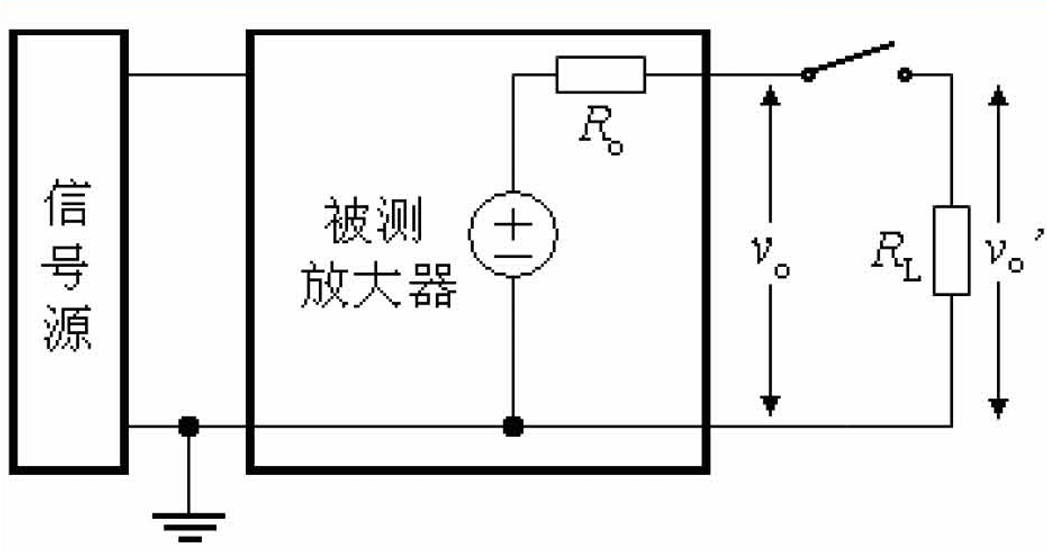
\includegraphics[width=0.4\textwidth, height=0.15\textheight]{16.png}
    \caption{输出电阻测量原理}
    \label{fig16}
\end{figure}

\begin{table}[H]
\centering
\caption{输出电阻测量数据}
\begin{tabular}{|c|c|c|c|c|}
\hline
$R_L$ (k$\Omega$) & $v_o$ (V) & $v_o'$ (V) & $R_o$(实测/k$\Omega$) & $R_o$ (理论/k$\Omega$)  \\
\hline
5.1 &382.28 & 193.58&4.971 &5.030 \\
\hline
\end{tabular}
\end{table}

\subsubsection*{6.2.5 频率特性测量}

（1）输入2kHz、10mV正弦信号，记录输出电压$V_{oP-P}$；

（2）计算0.707$V_{oP-P}$值；

（3）保持$v_i$幅度不变，改变频率至输出电压降至0.707倍，记录$f_L$、$f_H$；

（4）插入$C_u = 30pF$，测量$f_H(C_u)$。

\begin{table}[H]
\centering
\caption{截止频率测量数据}
\begin{tabular}{|c|c|c|c|}
\hline
 $f_L$ (Hz) & $f_H$ (Hz) & $f_H$ (Cu=30pF) (Hz) & 通频带$BW$ (Hz) \\
\hline
 34 &576k & 421k& 约576k/421k\\

\hline
\end{tabular}
\end{table}




\section*{七、数据分析与讨论}

将理论估算值（这里选用了仿真结果）与实验测量值的主要参数进行比较，发现除了下限频率$f_L$外，其他参数都与理论值相符合。至少说明了我们的参数计算、实验操作是没有大问题的，因为除了电容值是给定的，其余电阻取值是我们自己计算得出的。

\begin{table}[H]
\centering
\caption{理论计算、仿真结果与测量结果主要参数比较} 
\renewcommand{\arraystretch}{1.2}
\small
\begin{tabular}{|p{1.6cm}|p{1.4cm}|p{1.4cm}|p{1.4cm}|p{1.4cm}|p{1.4cm}|p{1.4cm}|p{1.8cm}|}
\hline
& $I_C$(mA) & $|A_V|$ &$R_i(\text{k}\Omega)$ &$R_o(\text{k}\Omega)$& $f_L$(Hz)& $f_H$(Hz)& $f_H(C_u)$(Hz)  \\
\hline
理论计算 &1.026 &20.35 &7.90 &5.10 &28.17 &-- &-- \\
\hline
仿真结果 &0.989 &19.940 &9.148 &5.030 &29.634 &578.57k & 453.46k \\
\hline
测量结果 &0.982 &19.358 &10.50&4.971 & 34 &576k &421k \\
\hline

\end{tabular}

\end{table}



\section*{八、结论}



\section*{九、心得与体会}

在本次实验中，我学会了

\end{document}